\chapter{PyTorch数据处理}
\label{cha:pytorch数据处理}

\section{数据处理工具箱概述}
\label{sec:pytorch_数据处理工具箱概述}
PyTorch提供了一系列数据处理工具箱，主要包括以下几个部分。
\begin{enumerate}[label=\arabic*)]
    \item torch.utils.data：数据加载工具箱，提供了Dataset、DataLoader等工具。
    \item torchvision：图形处理工具箱，提供了常用的数据集加载、数据预处理、图像处理等工具。
    \item torchaudio：音频处理工具箱，提供了音频数据加载、音频数据处理等工具。
    \item torchtext：文本处理工具箱，提供了文本数据加载、文本数据处理等工具。
\end{enumerate}

\section{utils.data}
\label{sec:pytorch_utils.data}
是torch.utils.data工具包，它包括以下4个类。
\begin{enumerate}[label=\arabic*)]
    \item Dataset ： 一个抽象类，其他数据集需要继承这个类，并且覆写其中的两个方法(\codeinline{\_\_getitem\_\_}、\codeinline{\_\_len\_\_})。

    \item (\textcolor{red}{\textbf{数据模块核心}})DataLoader：定义一个新的迭代器，实现批量(batch)读取，打乱数据(shuffle)并提供并行加速等功能。
    因为\codeinline{\_\_getitem\_\_}\textcolor{red}{\textbf{一次只能}}获取一个样本，
    所以通过\codeinline{torch.utils.data.DataLoader}来实现批量读取。

    \item \codeinline{random\_split}：把数据集随机拆分为给定长度的非重叠新数据集。
    \item \codeinline{*Sampler}：多种采样函数。
\end{enumerate}

dataset负责与磁盘打交道，将磁盘上的数据读取并预处理好，提供给DataLoader，
而DataLoader只需要关心如何组装成批数据，以及如何采样。
采样的体现是出现在传入getitem函数的索引，这里采样的规则可以通过sampler由用户自定义，
可以方便地实现均衡采样、随机采样、有偏采样、渐进式采样等。
\begin{figure}[htpb]
    \centering
    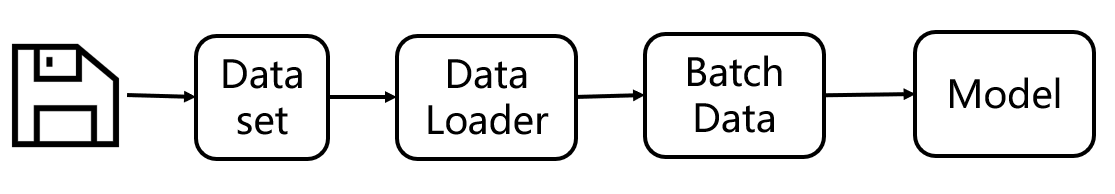
\includegraphics[width=0.6\textwidth]{part/人工智能/深度学习框架/pic/Pytorch/PyTorch数据处理/Dataset与DataLoader的关系.png}
    \caption{Dataset与DataLoader的关系}
    \label{fig:Dataset与DataLoader的关系}
\end{figure}


\subsection{Dataset 数据交互模块}
\label{subsec:pytorch_Dataset}
pytorch提供的torch.utils.data.Dataset类是一个抽象基类An abstract class representing a Dataset，供用户继承，
编写自己的dataset，实现对数据的读取。

在Dataset类的编写中\textcolor{red}{\textbf{必须}}要实现的两个函数是
\begin{enumerate}[label=\arabic*)]
    \item \codeinline{\_\_getitem\_\_}：
    通过给定索引(index)获取数据、标签或一个样本。
    然后实现从磁盘中读取数据，并进行预处理（包括online的数据增强），
    然后返回一个样本的数据。
    
    数据可以是包括模型需要的输入、标签，也可以是其他元信息，例如图片的路径。
    \codeinline{\_\_getitem\_\_}返回的数据会在dataloader中组装成一个batch。
    即，通常情况下是在dataloader中调用Dataset的\codeinline{\_\_getitem\_\_}函数获取一个样本。

    \item \codeinline{\_\_len\_\_}：返回数据集的长度。
\end{enumerate}


\begin{lstlisting}[style=pythonstyle]
# 导入需要的库
import torch
from torch.utils import data
import numpy as np

# 定义获取数据集的类
class TestDataset(data.Dataset): # 继承 Dataset，自定义数据集类
    def __init__(self):
        self.Data = np.asarray([[0, 1], [2, 3], [2, 1], [3, 4], [4, 5]])
        self.Label = np.asarray([0,1,3,5,2])

    # __getitem__方法用来获取数据集中第index个样本
    def __getitem__(self, index):
        # 把numpy转换为Tensor
        txt = torch.from_numpy(self.Data[index])
        label = torch.tensor(self.Label[index])
        return txt, label

    def __len__(self):
        return len(self.Data)

# 获取数据集中的数据
Test = TestDataset()
print(Test[2]) # 相当于调用 __getitem__(2) 方法
print(Test.__getitem__(2))
print(Test.__len__()) 
print(Test[0]) # 相当于调用 __getitem__(0) 方法
\end{lstlisting}
\begin{lstlisting}[style=demostyle,numbers=none] 
(tensor([2, 1]), tensor(3))
(tensor([2, 1]), tensor(3))  # 两者等价
5
(tensor([0, 1]), tensor(0))
\end{lstlisting}    

以上数据以元组格式返回，每次只返回一个样本。

\subsection{DataLoader 数据加载模块}
\label{subsec:pytorch_DataLoader}
实际上，Dataset只负责数据的抽取，一次调用\codeinline{\_\_getitem\_\_}只返回一个样本。
如果希望批量处理，同时进行数据打乱和并行加速等操作，
可选择\codeinline{DataLoader}。DataLoader的格式为：
\begin{lstlisting}[style=demostyle,numbers=none] 
data.DataLoader(
    dataset,        # 数据集
    batch_size=1,   # 批量大小
    shuffle=False,  # 是否打乱数据
    sampler=None,   # 样本抽样
    batch_sampler=None,  # 批量抽样
    num_workers=0,  # 并行线程数,0代表不使用多进程
    collate_fn=None,    # ：如何将多个样本数据拼接成一个批量，一般使用默认的拼接方式即可
    pin_memory=False,   # 是否将数据保存在锁页内存(pin_memory)区，
                        # pin_memory中的数据转到GPU会快一些。    
    drop_last=False,    # 是否丢弃最后一个不完整的 batch
                        # dataset中的数据个数可能不是batch_size的整数倍，
                        # 将drop_last设置为True时会将多出来且不足一个批量的数据丢弃。
    timeout=0,          # 加载数据超时时间
    worker_init_fn=None,    # 每个 worker 初始化函数
    multiprocessing_context=None,  # 多进程上下文
    generator=None, *, # 生成器
    prefetch_factor=2,  # 预取因子
    persistent_workers=False # 是否使用持久化工作进程
)   
\end{lstlisting} 

\begin{lstlisting}[style=pythonstyle]
# 导入需要的库
import torch
from torch.utils import data
import numpy as np

# 定义获取数据集的类
class TestDataset(data.Dataset): # 继承 Dataset，自定义数据集类
    def __init__(self):
        self.Data = np.asarray([[0, 1], [2, 3], [2, 1], [3, 4], [4, 5]])
        self.Label = np.asarray([0, 1, 0, 1, 2])

    def __getitem__(self, index):
        # 把numpy转换为Tensor
        txt = torch.from_numpy(self.Data[index])
        label = torch.tensor(self.Label[index])
        return txt, label

    def __len__(self):
        return len(self.Data)

# 获取数据集中的数据
Test = TestDataset()
#####################
# 1)单个获取
# print(Test[2]) # 相当于调用 __getitem__(2) 方法
# print(Test.__len__()) # 相当于调用 __len__() 方法    
# print(Test[0]) # 相当于调用 __getitem__(0) 方法

#####################
# 2)使用DataLoader加载数据
test_loader = data.DataLoader(Test, batch_size=3, shuffle=False, num_workers=2)
for i, data in enumerate(test_loader):
    inputs, labels = data
    print(f"Batch {i}:")
    print(f"数据：{inputs}")
    print(f"标签：{labels}\n")

print("-------------------------")
# 批量读取。我们可以像使用迭代器一样使用它，如对它进行循环操作。不过它不是迭代器，可以通过iter命令转换为迭代器。    
dataiter = iter(test_loader)
inputs, labels = next(dataiter)
print(f"数据：{inputs}")
print(f"标签：{labels}")
\end{lstlisting}

批量读取我们可以像使用迭代器一样使用它，如对它进行循环操作。
不过它不是迭代器，可以通过\codeinline{iter}命令转换为迭代器。

\begin{lstlisting}[style=demostyle,numbers=none] 
Batch 0:
数据：tensor([[0, 1],
        [2, 3],
        [2, 1]])
标签：tensor([0, 1, 0])

Batch 1:
数据：tensor([[3, 4],
        [4, 5]])
标签：tensor([1, 2])

-------------------------
数据：tensor([[0, 1],
        [2, 3],
        [2, 1]])
标签：tensor([0, 1, 0])
\end{lstlisting}

    
    

\section{torchvision 图形处理工具箱}
\label{sec:pytorch_torchvision}
torchvision包括4个类，各类的主要功能如下。
\begin{enumerate}[label=\arabic*)]
    \item datasets：提供常用的数据集加载，设计上都是继承\codeinline{torch.utils.data.Dataset},主要包括MNIST、CIFAR10/100. ImageNet. COCO 等。
    \item models：提供深度学习中各种经典的网络结构以及训练好的模型（如果要选择训练好的模型，则设置\codeinline{pretrained = True})，包括AlexNet、VGG系列、ResNet系列Inception系列等。
    \item transforms：常用的数据预处理操作，主要包括对\codeinline{Tensoi}及\codeinline{PIL Image}对象的操作。
    \item utils：含两个函数，一个是\codeinline{make\_grid},它能将多张图像拼接在一个网格中；另一个是\codeinline{savejmg},它能将\codeinline{Tensor}保存为图像。
\end{enumerate}

\subsection{torchvision安装}
\label{subsec:pytorch_torchvision安装}
torchvision是PyTorch的一个视觉处理工具包，独立于PyTorch,需要另外安装。
\begin{lstlisting}[style=demostyle,numbers=none] 
pip install torchvision
# 或者
conda install torchvision
\end{lstlisting}

\subsection{torchvision.datasets}
\label{subsec:pytorch_torchvision.datasets}

\subsection{torchvision.models}
\label{subsec:pytorch_torchvision.models}

\subsection{torchvision.transforms}
\label{subsec:pytorch_torchvision.transforms}
transforms提供了对PIL Image对象和Tensor对象的常用操作。

对 PIL Image 的操作包括：
\begin{enumerate}[label=\arabic*)]
    \item \codeinline{Scale/Resize}：调整图片尺寸，长宽比保持不变。
    \item \codeinline{CenterCrop}：从中心开始裁剪图片。
    \item \codeinline{RandomCrop}：随机裁剪。
    \item \codeinline{RandomSizeCrop}：随机尺寸裁剪。
    \item \codeinline{Pad}:填充。
    \item \codeinline{ToTensor}：将PIL Image对象转为Tensor，
    会自动将[0,255]归一化至[0,1]。
    \item \codeinline{RandomHorizontalFlip}：随机水平翻转,概率为0.5。
    \item \codeinline{RandomVerticalFlip}：随机垂直翻转,概率为0.5。
    \item \codeinline{ColorJitter}：调整亮度、对比度、饱和度和色相。
\end{enumerate}

对 Tensor 的操作包括：
\begin{enumerate}[label=\arabic*)]
    \item \codeinline{Normalize}：标准化。
    \item \codeinline{ToPILImage}：将Tensor转为PIL Image对象。
\end{enumerate}

如果要对数据集进行多个操作，可通过Compose将这些操作像管道一样拼接起来，
类似于\codeinline{nn.Sequential}

\begin{lstlisting}[style=demostyle,numbers=none] 
# 例如    
transforms.Compose([
    # 从图片中间裁剪出224*224的图片
    transforms.RandomResizedCrop(224),
    # 随机水平翻转，概率为0.5
    transforms.RandomHorizontalFlip(),
    # 将图片像素值归一化
    transforms.ToTensor(),
    # 标准化
    transforms.Normalize(mean=[0.485, 0.456, 0.406],
                         std=[0.229, 0.224, 0.225])
])
\end{lstlisting}    



\subsection{torchvision.utils}
\label{subsec:pytorch_torchvision.utils}









\section{可视化工具}
\label{sec:pytorch_可视化工具}
\subsection{TensorBoard}
\label{subsec:pytorch_tensorboard}
TensorBoard是Google TensorFlow的可视化工具，
可以记录训练数据、评估数据、网络结构、图像等，
并且可以在Web上展示，对于观察神经网络训练的过程非常有帮助。
PyTorch支持\codeinline{tensorboard\_logger}、\codeinline{visdom}等可视化工具。

TensorBoard 功能很强大，支持 scalar、image、figureA histogram、audio、text、
graph、onnx\_graph、embedding、 pr\_curve、videosummaries 等可视化方式。 

\subsubsection{安装}
\label{subsubsec:pytorch_tensorboard安装}
\begin{lstlisting}[style=demostyle,numbers=none] 
pip install tensorboard
\end{lstlisting}

\subsubsection{使用}
\label{subsubsec:pytorch_tensorboard使用}

执行下面命令
\begin{lstlisting}[style=demostyle,numbers=none] 
tensorboard --logdir=<event文件目录>
\end{lstlisting}

复制网址\url{http://localhost:6006/} 到浏览器中进行打开

\begin{enumerate}[label=\arabic*)]
    \item 如果conda环境下没有安装tensorboard，可以通过以下命令启动tensorboard。
    \begin{lstlisting}[style=demostyle,numbers=none] 
    tensorboard --logdir=/home/tony/Pratice/Python/Pytorch/NFEM --port 6006 --load_fast=false
    \end{lstlisting}

    \item 在tensorboard启动的过程中，可能发生的问题：

    6006端口被占用：
    \begin{lstlisting}[style=demostyle,numbers=none] 
    port 6006 was already in use 
    E0117 15:58:38.631224 MainThread program.py:260] TensorBoard attempted to bind to port 6006, but it was already in use
    TensorBoard attempted to bind to port 6006, but it was already in use
    \end{lstlisting}
    
    解决方法：修改端口为6007
    \begin{lstlisting}[style=demostyle,numbers=none] 
    tensorboard --logdir=your_dir --port=6007
    \end{lstlisting}
\end{enumerate}

\begin{lstlisting}[style=pythonstyle]
# 可视化神经网络  
# 导入需要的模块。  
import torch  
import torch.nn as nn  
import torch.nn.functional as F  
import torchvision  
from torch.utils.tensorboard import SummaryWriter  

import os
log_dir = os.getcwd()  # 或者指定一个相对于当前工作目录的子目录，如 'logs'  

# 1.构建神经网络。  
class Net(nn.Module):  
    def __init__(self):  
        super(Net, self).__init__()  
        self.conv1 = nn.Conv2d(1, 10, kernel_size=5)  
        self.conv2 = nn.Conv2d(10, 20, kernel_size=5)  
        self.conv2_drop = nn.Dropout2d()  
        self.fc1 = nn.Linear(320, 50)  
        self.fc2 = nn.Linear(50, 10)  
        self.bn = nn.BatchNorm2d(20)  
  
    def forward(self, x):  
        x = F.max_pool2d(self.conv1(x), 2)  
        x = F.relu(x) + F.relu(-x)  # 这里是双边ReLU，通常不常见，可能是个实验性设计  
        x = F.relu(F.max_pool2d(self.conv2_drop(self.conv2(x)), 2))  
        x = self.bn(x)  
        x = x.view(-1, 320)  
        x = F.relu(self.fc1(x))  
        x = F.dropout(x, training=self.training)  
        x = self.fc2(x)  
        x = F.softmax(x, dim=1)  
        return x  
  
# 2.把模型保存为图像  
# 1）定义输入。          
input_tensor = torch.rand(1, 1, 28, 28)  
# 2）实例化模型。  
model = Net()  
# 3）把模型保存为图像。  
with SummaryWriter(log_dir=log_dir, comment='Net') as w:  
    w.add_graph(model, (input_tensor, ))
\end{lstlisting}
\begin{lstlisting}[style=pythonstyle]
# 可视化损失函数
# 可视化损失值时需要用到add_scalar函数，这里利用一层全连接神经网络，训练一元二次函数的参数。
import torch
import torch.nn as nn
from torch.utils.tensorboard import SummaryWriter
import numpy as np

input_size = 1
output_size = 1
num_epoches = 60
learning_rate = 0.01

dtype = torch.FloatTensor
writer = SummaryWriter(log_dir='logs',comment='Linear')
np.random.seed(100) 
x_train = np.linspace(-1, 1, 100).reshape(100,1) 
y_train = 3*np.power(x_train, 2) +2+ 0.2*np.random.rand(x_train.size).reshape(100,1) 

model = nn.Linear(input_size, output_size)

criterion = nn.MSELoss()
optimizer = torch.optim.SGD(model.parameters(), lr=learning_rate)

for epoch in range(num_epoches):
    inputs = torch.from_numpy(x_train).type(dtype)
    targets = torch.from_numpy(y_train).type(dtype)

    output = model(inputs)
    loss = criterion(output, targets)

    optimizer.zero_grad()
    loss.backward()
    optimizer.step()
    # 保存loss的数据与epoch数值
    writer.add_scalar('训练损失值', loss, epoch)
\end{lstlisting}


